\chapter{Further Theorems of Continuation}\label{chap16}

\section{Theorem of Schwartz}\label{chap16:sec1}

We\pageoriginale have proved in Lecture 11, \S \ref{chap11:sec4} that if $\Lambda$ is a negative
sequence, $\Lambda = \big \{ - \lambda_n \big\}$ and $\sum
\dfrac{1}{\lambda_n} = \infty$, then $\mathscr{C}_\Lambda (I) =
\mathscr{C} (I)$. Conversely if $\sum \dfrac{1}{\lambda_n} < \infty$,
then $\mathscr{C}_\Lambda (I) \neq \mathscr{C}(I)$. Let us recall that
the function 
$$
D(w) = \prod_{1}^N \left(1 + \frac{w}{\lambda_n}\right) \prod^\infty_{N + 1}
\frac{\sin \pi w/ \lambda_n}{w/\lambda_n} 
$$
satisfies $D(\Lambda) = 0, D(u) = 0(\dfrac{1}{u^2})$ and $\big |D (w)
\big | < K e^{h|v|}$, where $h = \pi \sum\limits^{\infty}_{N+1}
\dfrac{1}{\lambda_n}$. 

Suppose $f \in \mathscr{C}_\Lambda (I), \Lambda = \{- \lambda_n \}$
and $\sum \dfrac{1}{\lambda_n} < \infty$. Then we shall prove that $f$
can be continued to a half-plane at the right, above and below $I$. 

We take $I = (- h, h)$ and $A_Z(w) = \sum e^{- \lambda Z} / D'
(\lambda) (w - \lambda)$, where $D(\lambda) = 0$. The idea is still to
define $A_Z(w)$ as an integral. To do this, we take a set of ``Cartan
circles'' $\Gamma$ constructed for a given $\in > 0$ and
$\Lambda$ (see Lecture \ref{chap14}). Let $w$ lie on a circle $\Gamma_1$
concentric to circle $\Gamma$ and of radius equal to $\in + $
radius of $\Gamma$. Consider the following expression: 
$$
A_Z (w) = \frac{1}{2 \pi i} \int \frac{e^{w' Z d w'}}{D(w') (w-w')},
w \varepsilon \text { one } \Gamma_1 
$$

\begin{figure}[H]
 \centerline{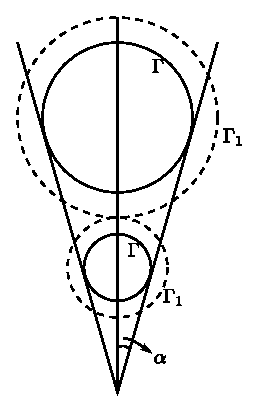
\includegraphics{vol15-figures/fig15-18.eps}}
\end{figure}

We have
$$
\big | e^{w' Z} \big | = e^{r R \cos (\varphi + \theta)}, Z = R e^{i
 \varphi}, w' = r e^{i \theta}. 
$$
\begin{figure}[H]
 \centerline{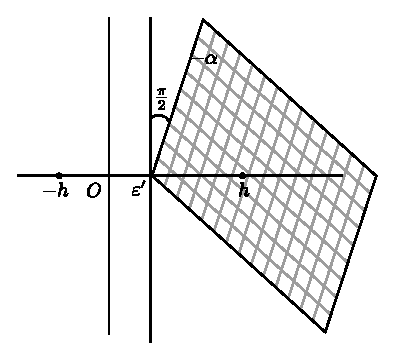
\includegraphics{vol15-figures/fig15-19.eps}}
\end{figure}

When $Z$ varies in an angle $\big | \arg (Z - \in ') \big | <<
\dfrac{\pi}{2} (\in ' > 0)$, one can choose $\in ' -$
and then the $\Gamma'$s so that $A_Z (w)$ is uniformly bounded in $Z$
on $\cup \Gamma_1$. Indeed if the ``Cartan circles''\pageoriginale $\Gamma$ are
contained in an angle $\big | \arg w - \dfrac{\pi}{2}\big| < \alpha$ and if
$\big | \arg (Z - \in ') \big | \le \pi / 2 - \alpha$ we have a
uniform majorization. Also by construction, $\alpha \to 0$ when
$\in \to 0$. Consider $w^2 M_Z (w) = A_Z (w) D(w)
w^2$. Outside the circles $\Gamma_1$ we have $\big | w^2 M_Z (w) \big
| < K_1 \big | w^2 D(w) \big |$. If $\in $ is small enough, it
follows, by lemma \ref{chap14:lem6}, lecture \ref{chap14}, that $\big | w^2 M_Z (w) \big | <
K_2 e^{h | v |}$ and also $\big | M_Z (w) \big | < K_2 e^{h |v |} $
uniformly in $Z$. Thus $M_Z (w) = A_z (w) D(w)$ is the Fourier
transform of a measure with support in $(- h, h)$. This enables us to
define $f(Z) = \int^h_{-h} f(z) d \mu_Z (z)$. Moreover, $\int \big | d
\mu_Z \big |$ is bounded when $\big | \arg (Z - \in ') \big |
\le \dfrac{\pi}{2} - \alpha$. So $f (Z)$ is uniformly approximated in
this angle by the same linear combinations of $e^{- \lambda_nZ}$
which approximate $f$ uniformly on $(- h, h)$. 

\begin{theorem*} % the
 If $\Lambda$ is an imaginary sequence $\big \{ i \lambda n \big\}$
 such that $\lambda_n>0$, $\sum \dfrac{1}{\lambda_n}< \infty$ every $f \in
 \mathscr{C}_\Lambda (I)$ is an analytic function, continuable into
 each right half - plane $Re z \ge x_o, x_o$ in the interior of
 $I$. In each angle, $\big | \arg (z - x_o) \big |< \beta <
 \dfrac{\pi}{2} (x_o$ in the interior of $I), \big | f (z) \big | <
 K \sup\limits_{x \in I} \big | f (x) \big |, K$ depending only on
 the angle. 
\end{theorem*}

\noindent
\textbf{Problem.} It would be interesting to have a half-plane $Re z
\le x_o$ instead of the angle, in the last statement. This is certainly
possible when $\Lambda$ is regular enough. Then, for a mean-periodic
function $f$ of spectrum $\Lambda$ we would have 
$$
\big | M(x) \big | = \sup_{Re z = x} \big | f (z) \big | = K \sup_{|
 \xi | < \eta} \big | f(x+ \xi ) \big | 
$$
a relation between the order of magnitude on the whole plane and on the line.

\section{Interpolation Results}\label{chap16:sec2}%sec 2

Suppose\pageoriginale $f \in \mathscr{H}_\Lambda (\Omega_c \cup \Omega_{-c})$. We
have seen that if $\Lambda$ is real and with finite $\bar{D}^.,
\Omega_c$ and $\Omega_{-c}$ being circles with centres $-c$ and $c$
and radii larger than $\pi \bar{D}^.$, we can continue $f$ into a
rectangle with vertices at $c$ and $-c$.Results of this type will
give us some indications about the domain of existence of the
continued function. 

Suppose $D(w)$ is an entire function of exponential type with
$D(\Lambda) = 0$ and let $\Omega$ be an open set containing the
conjugate diagram of $D$. We take two translates $\Omega_c$ and
$\Omega_{-c}$ of $\Omega$. We try to construct a measure $d \nu= d
\nu_{c, Z}(z)$ with support in $\Omega_{-c} \cup \Omega_c$ with the
aid of the measure $\mu$ such that we have $e^{\lambda Z} = \int e^{\lambda z }
d \nu$ whenever $\lambda \in \Lambda$. Then we can define $f (Z) = \int f(z)
d\nu_{c,Z} (z)$. We take $d \nu = d \mu_Z * (\delta_c - \delta_{-c})$,
where $\delta$ is the Dirac measure. $\mathscr{C} (d \nu) = M(w)
(e^{-wc}) = 2 M(w) Sh (cw)$. If we want the conjugate diagram of $M(w)$
in $\Omega$ we should expect $M(w) $ to have the same majorization as
$D(w)$. Let $M(w) = D(w) A(w)$. We suppose first that $D(w)$ and
$Sh(cw)$ have no common zeros. We construct $A(w)$ bounded in circles
of radius $R_j$ and on certain directions $\arg w = \theta \in
E$. Moreover, we want $2D (\lambda) Sh(c \lambda) A ( \lambda) =
e^{\lambda Z} $ for each $\lambda \in \Lambda$. For that we take the
following form of $A(w)$: 
$$
A(w) =\frac{e^{wZ}}{D(w) Sh(cw)} - \sum^\infty_{- \infty}
\frac{e^{\mu_nZ}}{D (\mu_n) Sh' (\mu_n c) (w - \mu_n)}, \mu_n =
\frac{i \pi n}{c}. 
$$

\noindent
Let $E$ be the set of points in $[ 0, 2 \pi ]$ where $\lim\limits_{r
 \to \infty} \inf \dfrac{\log \big | D(re^{i \theta}) \big |}{r} >
\in > 0$. 

In order to have the conjugate diagram of $M(w)$ in $\Omega$, it is
sufficient to have $E$ dense in $[0, 2 \pi ]$, $\arg (i/c ) \in E$
and $Z \in [ - c, c]$. 

Here\pageoriginale we give some results without details where this
method is applicable. 

\begin{theorem*}
 Let $C(w)$ be an entire function of exponential type with\break $C
 (\Lambda) = 0$ and the conjugate diagram of $C(w)$ contained in
 $\Omega$. Let the set $E (\in )$ of points $\theta$ for which
 $\lim\limits_{r \to \infty} \inf \dfrac{\log \big | C(r e^{i
  \theta}) \big |}{r} > - \in $ be dense in $(0, 2 \pi)$
 for every $\in > 0$. Then every function $f \in
 \mathscr{H}_\Lambda (\Omega_{-c} \cup \Omega_c)$ can be continued
 analytically along the segment $(-c, c)$. 
\end{theorem*}

We take $D(w) = C(w) \sin (\in w) Sh (\in w)$ and
apply the above method. 

As a corollary, we get the following result: if $G =
\bigcup\limits_{\zeta \in y} \Omega_\zeta$ and if $f \in 
\mathscr{H}_\Lambda (G)$, $f$ is analytically continuable in the
convex closure of $\mathscr{Y}$. 

A more interesting result is the following, which is more difficult to prove.

\begin{theorem*} % the
 Suppose $\Lambda$ and $\Omega$ satisfy the hypothesis of the last
 theorem. Let $\mathscr{Y}$ be a connected set containing $0$, and $G
 = \bigcup_{\zeta \in \mathscr{Y}} \Omega_\zeta$. If $f \in
 \mathscr{H}_\Lambda (\Omega)$ and $f \in \mathscr{H}(G)$, $f$ is
 analytically continuable in the convex closure of $\mathscr{Y}$. 
\end{theorem*}

From this theorem one can deduce that every analytic mean-periodic
function on the line is analytically continuable in a horizontal strip
(perhaps degenerated into a half-plane or the whole plane), such that
every segment of length $L$ (mean period related to $\Lambda$) on the
frontier of the strip, contains at least one singularity of $f$. 

For the proofs, see (Kahane 1, p. 100-104).

\section{Theorems of Leontiev}\label{chap16:sec3}%sec 3

In\pageoriginale (Leontiev) a method is given for the answer to the problem raised
in lecture \ref{chap13}, viz. whether continuation along a chain of translates
$\Omega_\zeta $ of $\Omega$, with $\zeta$ in a closed curve
$\mathscr{Y}$ containing 0, of a function $f \in \mathscr{H}_\Lambda
(\Omega)$, implies that $f$ is analytically continuable in the
interior of $\mathscr{Y}$. The answer is affirmative when $\Omega$ is
conveniently related to $\Lambda$. We sketch the method of Leontiev. 
\begin{figure}[H]
 \centerline{
\includegraphics{vol15-figures/fig15-20.eps}}
\end{figure}

Let $C(w) = \prod\limits_{1}^\infty \left(1 - \dfrac{w^2}{\lambda^2_n}\right) =
\mathscr{C} (d \alpha)$ and let 
$$
C_k (w) = \prod_{n = k}^{\infty} \left(1 -
\frac{w}{\lambda^2_n}\right) = \mathscr{C} (d \alpha_k). 
$$

Heuristically $C_k (w) \to 1$ when $k \to \infty$ and $d \alpha_k \to$
Dirac measure. 

More precisely, $\big | C_k(w) \big | < K e^{\pi |w| (\bar{D}^. +
 \in )}$ and $C_k (w) \to 1$ on every compact set. Then, if
$\Gamma$ is a curve around the disc $|z| < \pi (\bar{D}^. +
\in )$ the Laplace-Borel transform of $C_k (w)$, denoted by
$\varphi_k (z)$, tends uniformly on $\Gamma$ to
$\dfrac{1}{z}$. Suppose $\Omega \supset \Gamma$, and $f \in
\mathscr{H}_\Lambda (\Omega)$; then the Dirichlet polynomial $f_k (z)
= \dfrac{1}{2 \pi i} \int_\Gamma f(z + \zeta) \varphi_k (\zeta) d
\zeta$ tends uniformly to $f(z)$ when $\big | z \big |$ is small
enough. 

If we suppose also $f \in \mathscr{H} (G), G = \bigcup\limits_{\zeta
 \in \mathscr{Y}} \Omega_\zeta$, then $f_k (z)$ is defined by the
same formula in a neighbourhood of $\mathscr{Y}$, so it is bounded and
tends uniformly to $f(z) $ on $\mathscr{Y}$. Hence 

\begin{theorem*} % the
 Suppose\pageoriginale $\Lambda$ is a symmetrical sequence $\big \{ \pm \lambda_n
 \big\}$ such that $\left \{ \big | \lambda_n \big | \right\}$ has a
 mean upper density $\bar{D}^.$, $\Omega$ is an open set containing $|
 z | \le \pi \bar{D}^., \mathscr{Y}$ is a closed curve passing through
 $0, ~ G = \bigcup\limits_{\zeta \in \mathscr{Y}} \Omega_\zeta$, and
 $H$ is the interior of $\mathscr{Y}$. Then, every $f \in
 \mathscr{H}_\Lambda (\Omega)$ which is analytically continuable in
 $G$ can be continued in $H$ as a function $\in \mathscr{H}_\Lambda
 (H)$. 
\end{theorem*}

\begin{coro*} %coro
 If $\dfrac{n}{\lambda_n} \to 0$, the domain of existence of every $f
 \in \mathscr{H}_\Lambda (H)$ is simply-connected. 
\end{coro*}

One can prove more, viz. the following result of Leontiev (stated
partly by $G$. Polya); 
\begin{theorem*} % the
 If $\dfrac{n}{\lambda_n} \to 0$, the domain of existence of every $f
 \in \mathscr{H}_\Lambda (\Omega)$ is convex. 
\end{theorem*}

For the proof, see (Leontiev).
